\documentclass[aspectratio=169, 10pt]{beamer}

% --- Packages ---
\usepackage[utf8]{inputenc}
\usepackage{tikz}
\usepackage{pgfplots}
\usepackage{amsmath, amssymb, amsfonts}
\usepackage{booktabs}
\usepackage{bm}
\usepackage{xcolor}
\usetikzlibrary{arrows.meta, calc, positioning, shapes.geometric, decorations.pathreplacing, backgrounds, fit, shadows, patterns, shapes.arrows, angles, quotes}
\pgfplotsset{compat=1.17}

% NYU Colors
\definecolor{nyupurple}{RGB}{87,46,140}
\definecolor{nyuheader}{RGB}{172,159,195}
\definecolor{nyufooter}{RGB}{189,178,211}

% Theme
\usetheme{default}
\setbeamertemplate{navigation symbols}{}

% Itemize
\setbeamercolor{itemize item}{fg=nyupurple}
\setbeamercolor{itemize subitem}{fg=nyupurple}
\setbeamercolor{itemize subsubitem}{fg=nyupurple}
\setbeamertemplate{itemize item}{\textbullet}
\setbeamertemplate{itemize subitem}{\textbullet}
\setbeamertemplate{itemize subsubitem}{\textbullet}

% Blocks
\setbeamercolor{block title}{fg=white, bg=nyupurple}
\setbeamercolor{block body}{fg=black, bg=nyuheader!30}
\setbeamercolor{block title alerted}{fg=white, bg=red!70}
\setbeamercolor{block body alerted}{fg=black, bg=red!10}
\setbeamercolor{block title example}{fg=white, bg=green!50!black}
\setbeamercolor{block body example}{fg=black, bg=green!10}

% Diagram colors
\definecolor{darkblue}{RGB}{0,51,102}
\definecolor{brightblue}{RGB}{0,102,204}
\definecolor{lightblue}{RGB}{153,204,255}
\definecolor{darkgreen}{RGB}{0,102,51}
\definecolor{accentred}{RGB}{192,0,0}
\definecolor{accentgreen}{RGB}{0,128,0}
\definecolor{accentorange}{RGB}{255,128,0}

% Commands
\newcommand{\vect}[1]{\boldsymbol{#1}}
\newcommand{\mat}[1]{\mathbf{#1}}
\newcommand{\xv}{\mathbf{x}}
\newcommand{\uv}{\mathbf{u}}
\newcommand{\xdot}{\dot{\mathbf{x}}}

% Header
\makeatletter
\setbeamertemplate{frametitle}{%
    \nointerlineskip%
    \begin{beamercolorbox}[wd=\paperwidth,ht=0.7cm,dp=0.15cm,rightskip=0.5cm]{frametitle}
        \hspace{0.3cm}\usebeamerfont{frametitle}\insertframetitle%
        \hfill%
        \raisebox{0.08cm}{{\bfseries\sffamily\color{nyupurple}NYU}}%
    \end{beamercolorbox}%
}
\makeatother
\setbeamercolor{frametitle}{fg=black, bg=nyuheader}
\setbeamerfont{frametitle}{size=\large}

% Footer
\setbeamertemplate{footline}{%
    \begin{tikzpicture}[remember picture, overlay]
        \fill[nyufooter] ([yshift=0.6cm]current page.south west) rectangle ([xshift=5cm]current page.south east);
        \fill[nyufooter!70] ([yshift=0.6cm, xshift=5cm]current page.south west) rectangle ([xshift=10.5cm]current page.south east);
        \fill[nyufooter!40] ([yshift=0.6cm, xshift=10.5cm]current page.south west) rectangle (current page.south east);
        \node[anchor=west, font=\small] at ([xshift=0.3cm, yshift=0.3cm]current page.south west) {Dr.\ Aliasghar Arab};
        \node[anchor=center, font=\small] at ([yshift=0.3cm]current page.south) {Autonomous Mobile Robots};
        \node[anchor=east, font=\small] at ([xshift=-0.3cm, yshift=0.3cm]current page.south east) {LECTURE 7 -- FALL 2025 \quad \insertframenumber{} / \inserttotalframenumber};
    \end{tikzpicture}%
}

% Title page
\defbeamertemplate*{title page}{customized}[1][]
{
    \begin{tikzpicture}[remember picture, overlay]
        \node[anchor=north east] at ([xshift=-0.8cm, yshift=-0.8cm]current page.north east) {%
            {\bfseries\sffamily\Large\color{nyupurple}NYU}%
            {\sffamily\normalsize\color{black}\ \ TANDON SCHOOL OF ENGINEERING}%
        };
    \end{tikzpicture}
    
    \vspace{2cm}
    \centering
    {\Large\bfseries\inserttitle\par}
    \vspace{0.3cm}
    {\insertsubtitle\par}
    \vspace{1cm}
    {\insertauthor\par}
    \vspace{0.3cm}
    {\small\insertinstitute\par}
    \vspace{0.5cm}
    {\insertdate\par}
}

% Title info
\title{Autonomous Mobile Robots}
\subtitle{Lecture 7: Model Predictive Control and Safety-Critical Control}
\author{Dr.\ Aliasghar Arab}
\institute{NYU Tandon School of Engineering}
\date{Fall 2025}

\begin{document}

% ================================================================
% TITLE SLIDE
% ================================================================
{
\setbeamertemplate{footline}{}
\begin{frame}[plain]
\titlepage
\end{frame}
}

% ================================================================
% LECTURE OVERVIEW
% ================================================================
\begin{frame}{Lecture Overview}

\textbf{Topics Covered:}

\vspace{0.4cm}

\begin{itemize}
    \item The Fundamental Control Problem: Performance vs.\ Safety
    
    \vspace{0.3cm}
    
    \item Nonlinear Model Predictive Control (NMPC)
    
    \vspace{0.3cm}
    
    \item Control Lyapunov Functions (CLF) for Stability
    
    \vspace{0.3cm}
    
    \item Control Barrier Functions (CBF) for Safety
    
    \vspace{0.3cm}
    
    \item Lie Derivatives and Computational Tractability
    
    \vspace{0.3cm}
    
    \item CLF-CBF Quadratic Programming (QP)
    
    \vspace{0.3cm}
    
    \item Two-Layer Architecture: NMPC + ASIF
\end{itemize}

\end{frame}

% ================================================================
% PART 1: THE FUNDAMENTAL CONTROL PROBLEM
% ================================================================
\section{The Fundamental Control Problem}

\begin{frame}{The Fundamental Control Problem}

\begin{center}
{\Large How do we guarantee both \textbf{performance} and \textbf{safety}?}
\end{center}

\vspace{0.5cm}

\begin{columns}[T]
\column{0.48\textwidth}
\begin{block}{Liveness (Performance)}
\begin{itemize}
    \item Reach target destinations
    \vspace{0.2cm}
    \item Minimize tracking error
    \vspace{0.2cm}
    \item Optimize metrics
\end{itemize}
\end{block}

\column{0.48\textwidth}
\begin{block}{Safety}
\begin{itemize}
    \item Collision avoidance
    \vspace{0.2cm}
    \item Respect physical limits
    \vspace{0.2cm}
    \item Maintain stability
\end{itemize}
\end{block}
\end{columns}

\vspace{0.5cm}

\begin{alertblock}{Challenge}
These objectives often \textbf{conflict}. Traditional methods struggle when safety and performance contradict.
\end{alertblock}

\end{frame}

% ================================================================
\begin{frame}{System Formulation}

\textbf{Control Objective:} Navigate to goal $\xv_d^*$

\vspace{0.4cm}

\begin{columns}[T]
\column{0.45\textwidth}
\textbf{State Variables:}
\begin{itemize}
    \item Position: $x, y$
    \vspace{0.2cm}
    \item Orientation: $\theta$
    \vspace{0.2cm}
    \item Velocities: $v, \omega$
\end{itemize}

\vspace{0.4cm}

\textbf{State Vector:}
\[
\mat{X} = \begin{bmatrix} x \\ y \\ \theta \\ v \\ \omega \end{bmatrix}
\]

\column{0.5\textwidth}
\centering
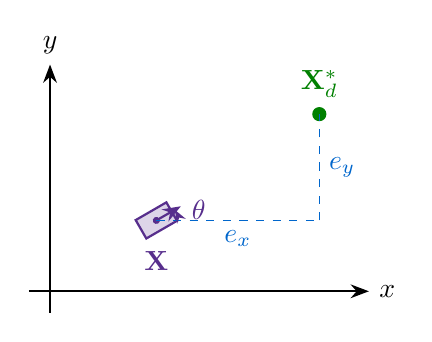
\begin{tikzpicture}[scale=0.9, >=Stealth]
    % Coordinate axes
    \draw[thick, ->] (-0.3,0) -- (4.5,0) node[right] {$x$};
    \draw[thick, ->] (0,-0.3) -- (0,3.2) node[above] {$y$};
    
    % Goal position
    \fill[accentgreen] (3.8,2.5) circle (0.1);
    \node[accentgreen, above] at (3.8,2.6) {$\mat{X}_d^*$};
    
    % Robot
    \begin{scope}[shift={(1.5,1)}, rotate=30]
        \draw[thick, nyupurple, fill=nyupurple!20] (-0.25,-0.15) rectangle (0.25,0.15);
        \draw[->, thick, nyupurple] (0,0) -- (0.4,0);
        \fill[nyupurple] (0,0) circle (0.05);
    \end{scope}
    \node[nyupurple, below] at (1.5,0.7) {$\mat{X}$};
    
    % Error vectors
    \draw[dashed, brightblue] (1.5,1) -- (3.8,1) node[midway, below] {$e_x$};
    \draw[dashed, brightblue] (3.8,1) -- (3.8,2.5) node[midway, right] {$e_y$};
    
    % Angle arc
    \draw[nyupurple, ->] (1.8,1) arc (0:30:0.3);
    \node[nyupurple] at (2.1,1.15) {$\theta$};
\end{tikzpicture}
\end{columns}

\end{frame}

% ================================================================
\begin{frame}{Mathematical Framework}

\textbf{System Dynamics:}
\begin{equation}
\dot{\mat{X}} = f(\mat{X}, \uv)
\end{equation}

\vspace{0.3cm}

\begin{itemize}
    \item $\mat{X}$: State vector (system configuration)
    \vspace{0.2cm}
    \item $\uv$: Control input (actuator commands)
    \vspace{0.2cm}
    \item $f$: Nonlinear dynamics (system physics)
\end{itemize}

\vspace{0.5cm}

\textbf{Output Equation:}
\[
y = h(\mat{X})
\]

Often only certain states matter (e.g., position: $y = [x, y]^T$)

\end{frame}

% ================================================================
\begin{frame}{Mathematical Framework (cont.)}

\textbf{With Disturbances:}
\[
\dot{\mat{X}} = f(\mat{X}, \uv) + d(t)
\]

\vspace{0.5cm}

We assume perfect models initially, then address robustness later.

\vspace{0.5cm}

\begin{block}{Key Insight}
The disturbance term $d(t)$ captures:
\begin{itemize}
    \item Unmodeled dynamics
    \vspace{0.2cm}
    \item External forces (wind, terrain)
    \vspace{0.2cm}
    \item Sensor noise and measurement errors
\end{itemize}
\end{block}

\end{frame}

% ================================================================
% PART 2: FROM CLASSICAL TO OPTIMAL CONTROL
% ================================================================
\section{Optimal Control Formulation}

\begin{frame}{From Classical to Optimal Control}

\begin{columns}[T]
\column{0.48\textwidth}
\textbf{Classical Approach:}

\vspace{0.3cm}

Design $\uv = k(\xv)$ using:
\begin{itemize}
    \item Linearization
    \vspace{0.2cm}
    \item Pole placement
    \vspace{0.2cm}
    \item Lyapunov methods
\end{itemize}

\vspace{0.3cm}

\textit{Stable but limited constraint handling}

\column{0.48\textwidth}
\textbf{Optimal Control:}

\vspace{0.3cm}

Formulate as optimization:
\begin{itemize}
    \item Explicit performance metric
    \vspace{0.2cm}
    \item Systematic constraints
    \vspace{0.2cm}
    \item Handles nonlinearity
\end{itemize}

\vspace{0.3cm}

\textit{Flexible but computationally intensive}
\end{columns}

\vspace{0.5cm}

\begin{block}{Optimal Control Problem}
\[
\min_{\uv} \quad J(\xv, \uv)
\]
subject to: dynamics, input limits, state constraints
\end{block}

\end{frame}

% ================================================================
\begin{frame}{The Cost Function}

Cost function $J$ defines \textbf{optimal behavior}

\vspace{0.4cm}

\begin{columns}[T]
\column{0.55\textwidth}
\textbf{Standard Components:}

\vspace{0.3cm}

\begin{enumerate}
    \item \textbf{Tracking error:} $e^T Q e$ where $e = \xv - \xv_d$
    
    \vspace{0.3cm}
    
    \item \textbf{Control effort:} $\int_0^T \uv^T R \uv \, dt$
    
    \vspace{0.3cm}
    
    \item \textbf{Constraint penalties:} Soft penalties for violations
\end{enumerate}

\vspace{0.4cm}

Can construct $J$ to also serve as Lyapunov function

\column{0.4\textwidth}
\centering
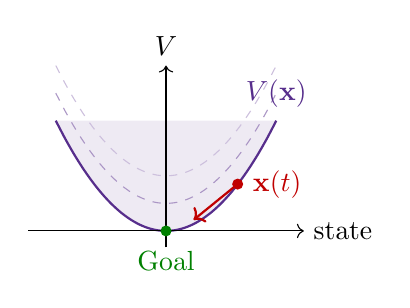
\begin{tikzpicture}[scale=0.7]
    % Bowl shape
    \draw[thick, nyupurple, fill=nyupurple!10] plot[smooth, domain=-2:2] (\x, {0.5*\x*\x});
    \draw[dashed, nyupurple!50] plot[smooth, domain=-2:2] (\x, {0.5*\x*\x + 0.5});
    \draw[dashed, nyupurple!30] plot[smooth, domain=-2:2] (\x, {0.5*\x*\x + 1});
    
    % Axes
    \draw[->] (-2.5,0) -- (2.5,0) node[right] {state};
    \draw[->] (0,-0.3) -- (0,3) node[above] {$V$};
    
    % Goal point
    \fill[accentgreen] (0,0) circle (0.1);
    \node[accentgreen, below] at (0,-0.2) {Goal};
    
    % Current state
    \fill[accentred] (1.3,0.85) circle (0.1);
    \node[accentred, right] at (1.4,0.85) {$\xv(t)$};
    
    % Arrow showing descent
    \draw[->, thick, accentred] (1.3,0.85) -- (0.5,0.2);
    
    \node[nyupurple] at (2,2.5) {$V(\xv)$};
\end{tikzpicture}
\end{columns}

\end{frame}

% ================================================================
\begin{frame}{Constraints: Formalizing Safety}

\begin{columns}[T]
\column{0.48\textwidth}
\textbf{Input Constraints:} $\uv \in \mathcal{U}_a$

\vspace{0.3cm}

Physical actuator limits:
\begin{itemize}
    \item Torque bounds
    \vspace{0.2cm}
    \item Velocity limits
    \vspace{0.2cm}
    \item Power constraints
\end{itemize}

\vspace{0.5cm}

\textbf{State Constraints:} $\xv \in \mathcal{X}_s$

\vspace{0.3cm}

Safety requirements:
\begin{itemize}
    \item Obstacle avoidance
    \vspace{0.2cm}
    \item Lane boundaries
    \vspace{0.2cm}
    \item Stability regions
\end{itemize}

\column{0.48\textwidth}
\centering
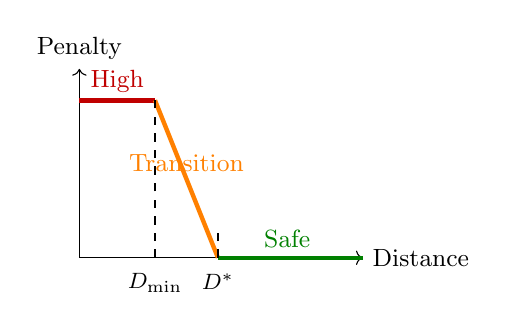
\begin{tikzpicture}[scale=0.8]
    % Axes
    \draw[->] (0,0) -- (4.5,0) node[right, font=\small] {Distance};
    \draw[->] (0,0) -- (0,3) node[above, font=\small] {Penalty};
    
    % High penalty region
    \draw[ultra thick, accentred] (0,2.5) -- (1.2,2.5);
    \node[accentred, font=\small] at (0.6,2.8) {High};
    
    % Transition region
    \draw[ultra thick, accentorange, domain=1.2:2.2, smooth] plot (\x, {2.5 - 2.5*(\x-1.2)});
    \node[accentorange, font=\small] at (1.7,1.5) {Transition};
    
    % Safe region
    \draw[ultra thick, accentgreen] (2.2,0) -- (4.5,0);
    \node[accentgreen, font=\small] at (3.3,0.3) {Safe};
    
    % Boundaries
    \draw[dashed] (1.2,0) -- (1.2,2.5);
    \node[below, font=\footnotesize] at (1.2,-0.1) {$D_{\min}$};
    \draw[dashed] (2.2,0) -- (2.2,0.5);
    \node[below, font=\footnotesize] at (2.2,-0.1) {$D^*$};
\end{tikzpicture}

\vspace{0.3cm}

\textbf{Implementation:}

\textbf{Hard:} Strict inequality constraints

\textbf{Soft:} Penalty functions in cost
\end{columns}

\end{frame}

% ================================================================
% PART 3: NMPC
% ================================================================
\section{Nonlinear Model Predictive Control}

\begin{frame}{NMPC vs MPPI}

\begin{columns}[T]
\column{0.48\textwidth}
\begin{block}{NMPC}
\textbf{Deterministic} optimization

\vspace{0.2cm}

\begin{itemize}
    \item Explicit system model
    \vspace{0.2cm}
    \item Gradient-based methods
    \vspace{0.2cm}
    \item Local optimum
    \vspace{0.2cm}
    \item Precise when model accurate
\end{itemize}
\end{block}

\column{0.48\textwidth}
\begin{block}{MPPI}
\textbf{Probabilistic} sampling

\vspace{0.2cm}

\begin{itemize}
    \item Monte Carlo evaluation
    \vspace{0.2cm}
    \item Tests many trajectories
    \vspace{0.2cm}
    \item Global search capability
    \vspace{0.2cm}
    \item Robust to model errors
\end{itemize}
\end{block}
\end{columns}

\vspace{0.5cm}

\centering
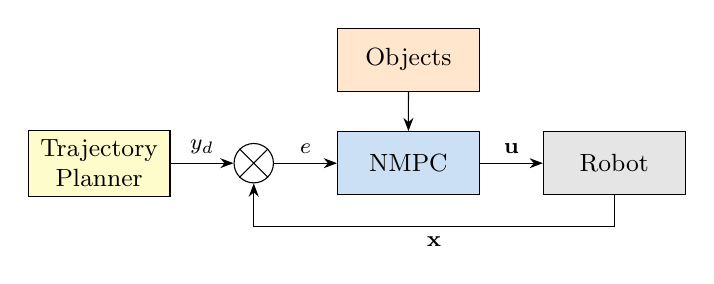
\begin{tikzpicture}[scale=0.8, >=Stealth,
    block/.style={draw, rectangle, minimum width=1.8cm, minimum height=0.8cm, align=center, font=\small}]
    \node[block, fill=yellow!20] (planner) {Trajectory\\Planner};
    \node[draw, circle, minimum size=0.5cm, right=0.8cm of planner] (sum) {};
    \draw (sum.north west) -- (sum.south east);
    \draw (sum.north east) -- (sum.south west);
    \node[block, fill=brightblue!20, right=0.8cm of sum] (nmpc) {NMPC};
    \node[block, fill=gray!20, right=0.8cm of nmpc] (robot) {Robot};
    \node[block, fill=accentorange!20, above=0.5cm of nmpc] (obj) {Objects};
    
    \draw[->] (planner) -- node[above, font=\footnotesize] {$y_d$} (sum);
    \draw[->] (sum) -- node[above, font=\footnotesize] {$e$} (nmpc);
    \draw[->] (nmpc) -- node[above, font=\footnotesize] {$\uv$} (robot);
    \draw[->] (obj) -- (nmpc);
    \draw[->] (robot.south) -- ++(0,-0.5) -| node[pos=0.25, below, font=\footnotesize] {$\xv$} (sum.south);
\end{tikzpicture}

\end{frame}

% ================================================================
\begin{frame}{NMPC: Prediction-Based Control}

\textbf{Core Concept:} Control the present by optimizing the predicted future

\vspace{0.4cm}

\begin{block}{NMPC Algorithm}
\textbf{At each time step:}
\begin{enumerate}
    \item Measure current state $\xv(t)$
    \vspace{0.2cm}
    \item Predict evolution over horizon $P$ (1-2 seconds)
    \vspace{0.2cm}
    \item Optimize control sequence $\{\uv_t, \uv_{t+1}, \ldots, \uv_{t+P}\}$
    \vspace{0.2cm}
    \item Apply \textbf{only first control} $\uv_t$
    \vspace{0.2cm}
    \item Repeat at next time step
\end{enumerate}
\end{block}

\end{frame}

% ================================================================
\begin{frame}{NMPC: Mathematical Formulation}

\textbf{Forward Simulation:}
\[
\xv_{k+1} = \xv_k + \Delta t \cdot f(\xv_k, \uv_k)
\]

\vspace{0.5cm}

\textbf{Objective:}
\[
\min_{\{\uv_k\}} J = \sum_{k=t}^{t+P} \ell(\xv_k, \uv_k)
\]

\vspace{0.3cm}

where $\ell(\xv_k, \uv_k)$ is the stage cost (tracking error + control effort)

\end{frame}

% ================================================================
\begin{frame}{Understanding Prediction Horizon}

\centering
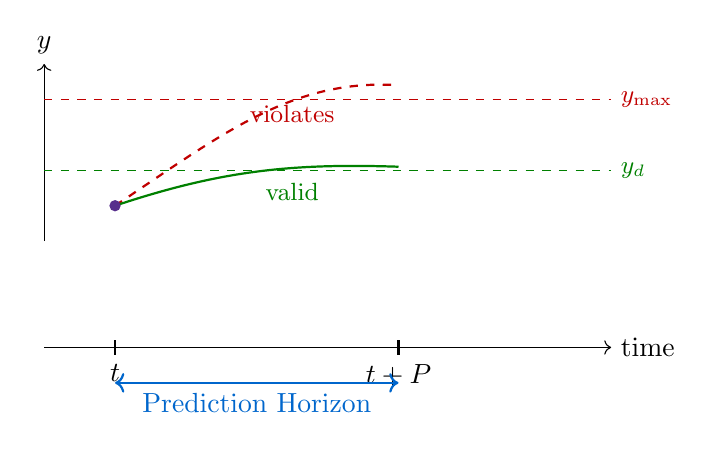
\begin{tikzpicture}[scale=0.9]
    % Time axis
    \draw[->] (0,0) -- (8,0) node[right] {time};
    \draw[thick] (1,0.1) -- (1,-0.1) node[below] {$t$};
    \draw[thick] (5,0.1) -- (5,-0.1) node[below] {$t+P$};
    \draw[<->, brightblue, thick] (1,-0.5) -- (5,-0.5) node[midway, below] {Prediction Horizon};
    
    % State evolution
    \draw[->] (0,1.5) -- (0,4) node[above] {$y$};
    
    % Constraints
    \draw[dashed, accentred] (0,3.5) -- (8,3.5) node[right, font=\small] {$y_{\max}$};
    \draw[dashed, accentgreen] (0,2.5) -- (8,2.5) node[right, font=\small] {$y_d$};
    
    % Violating trajectory
    \draw[thick, accentred, dashed] (1,2) .. controls (2.5,3) and (3.5,3.8) .. (5,3.7);
    \node[accentred, font=\small] at (3.5,3.3) {violates};
    
    % Valid trajectory
    \draw[thick, accentgreen] (1,2) .. controls (2.5,2.5) and (3.5,2.6) .. (5,2.55);
    \node[accentgreen, font=\small] at (3.5,2.2) {valid};
    
    % Current state
    \fill[nyupurple] (1,2) circle (0.08);
\end{tikzpicture}

\vspace{0.5cm}

\begin{columns}[T]
\column{0.48\textwidth}
\textbf{At time $t$:}
\begin{itemize}
    \item Current state: $\xv(t)$
    \item Horizon: $P$ time steps
    \item Test control sequences
    \item Generate predictions
\end{itemize}

\column{0.48\textwidth}
\textbf{Selection criteria:}
\begin{itemize}
    \item Minimizes cost $J$
    \item Satisfies constraints
    \item Approaches $y_d$
    \item Smooth dynamics
\end{itemize}
\end{columns}

\end{frame}

% ================================================================
\begin{frame}{NMPC Design Parameters}

\begin{block}{Critical Choices}
\begin{enumerate}
    \item \textbf{Problem Formulation:} Deterministic vs probabilistic, time discretization
    
    \vspace{0.3cm}
    
    \item \textbf{Objective Function:} Quadratic error? Time-optimal? CLF-based?
    
    \vspace{0.3cm}
    
    \item \textbf{Constraints:} Hard (inequality) vs soft (penalty)
    
    \vspace{0.3cm}
    
    \item \textbf{Optimization Solver:} Gradient descent, SQP, interior point
    
    \vspace{0.3cm}
    
    \item \textbf{Derivative Computation:} Analytical (fast) vs numerical (general)
\end{enumerate}
\end{block}

\end{frame}

% ================================================================
\begin{frame}{Example: Autonomous Racing}

\begin{columns}[T]
\column{0.48\textwidth}
\textbf{High-Speed Vehicle Control}

\vspace{0.3cm}

\textbf{Objectives:}
\begin{itemize}
    \item Minimize lap time
    \item Track centerline
    \item Allow controlled drift
\end{itemize}

\vspace{0.4cm}

\textbf{Safety Constraint:}
\begin{itemize}
    \item Prevent spinout
    \item Maintain stability
\end{itemize}

\vspace{0.4cm}

\textbf{Cost Function:}
\[
J = e_{\text{lat}}^2 + \dot{e}_{\text{lat}}^2 + e_\theta^2 + \text{penalties}
\]

\column{0.48\textwidth}
\textbf{Implementation:}
\begin{itemize}
    \item Nonlinear conjugate gradient
    \vspace{0.2cm}
    \item Numerical derivatives
    \vspace{0.2cm}
    \item Real-time embedded
    \vspace{0.2cm}
    \item Stability as barrier function
\end{itemize}

\vspace{0.5cm}

\begin{block}{Note}
Commercial cruise control uses similar formulations
\end{block}
\end{columns}

\end{frame}

% ================================================================
\begin{frame}{NMPC Challenges}

\begin{columns}[T]
\column{0.48\textwidth}
\textbf{Strengths:}
\begin{itemize}
    \item Handles nonlinearity
    \vspace{0.2cm}
    \item Explicit constraints
    \vspace{0.2cm}
    \item Performance optimization
    \vspace{0.2cm}
    \item Future prediction
\end{itemize}

\vspace{0.4cm}

\textbf{Limitations:}
\begin{itemize}
    \item High computational cost
    \vspace{0.2cm}
    \item Non-convex optimization
    \vspace{0.2cm}
    \item No real-time guarantees
    \vspace{0.2cm}
    \item Local optima
\end{itemize}

\column{0.48\textwidth}
\centering
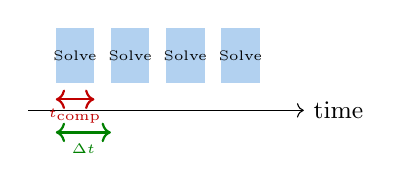
\begin{tikzpicture}[scale=0.7]
    \draw[->] (0,0) -- (5,0) node[right, font=\small] {time};
    
    % Computation blocks
    \foreach \x in {0.5, 1.5, 2.5, 3.5} {
        \fill[brightblue!30] (\x,0.5) rectangle (\x+0.7,1.5);
        \node[font=\tiny] at (\x+0.35,1) {Solve};
    }
    
    % Timing annotations
    \draw[<->, accentred, thick] (0.5,0.2) -- (1.2,0.2);
    \node[accentred, font=\tiny] at (0.85,-0.1) {$t_{\text{comp}}$};
    
    \draw[<->, accentgreen, thick] (0.5,-0.4) -- (1.5,-0.4);
    \node[accentgreen, font=\tiny] at (1,-0.7) {$\Delta t$};
\end{tikzpicture}

\vspace{0.4cm}

\textbf{Timing Constraint:}

Must satisfy:
\[
t_{\text{compute}} < \Delta t_{\text{control}}
\]
\end{columns}

\vspace{0.3cm}

\textbf{Solution:} Use NMPC for performance (slower), safety filter (fast)

\end{frame}

% ================================================================
% PART 4: CONTROL LYAPUNOV FUNCTIONS
% ================================================================
\section{Control Lyapunov Functions}

\begin{frame}{The Stability Question}

\textbf{Problem:} How do we \textit{guarantee} the system reaches its goal?

\vspace{0.5cm}

\begin{block}{Lyapunov Stability Theory}
For $\dot{\xv} = f(\xv)$, equilibrium $\xv^*$ is \textbf{stable} if $\exists V(\xv)$:

\vspace{0.3cm}

\begin{enumerate}
    \item $V(\xv) > 0$ for all $\xv \neq \xv^*$ \quad (positive definite)
    
    \vspace{0.2cm}
    
    \item $V(\xv^*) = 0$ \quad (zero at equilibrium)
    
    \vspace{0.2cm}
    
    \item $\dot{V}(\xv) \leq 0$ \quad (non-increasing)
\end{enumerate}
\end{block}

\vspace{0.4cm}

\textbf{Interpretation:} $V(\xv)$ is an ``energy function'' that monotonically decreases, guaranteeing convergence

\end{frame}

% ================================================================
\begin{frame}{Control Lyapunov Functions}

\textbf{Extension to Controlled Systems:} $\dot{\xv} = f(\xv, \uv)$

\vspace{0.5cm}

\begin{block}{CLF Definition}
Function $V(\xv)$ is a \textbf{CLF} if:

\vspace{0.3cm}

\begin{enumerate}
    \item $V$ is positive definite with $V(\xv_d) = 0$
    
    \vspace{0.2cm}
    
    \item For any $\xv \neq \xv_d$, $\exists \uv$ such that:
\end{enumerate}

\vspace{0.2cm}

\begin{equation}
\dot{V}(\xv, \uv) \leq -\gamma V(\xv), \quad \gamma > 0
\end{equation}
\end{block}

\vspace{0.4cm}

Transforms stability analysis into \textbf{control design tool}

\vspace{0.3cm}

Condition $\dot{V} \leq -\gamma V$ guarantees \textbf{exponential convergence}

\end{frame}

% ================================================================
\begin{frame}{CLF Example: Position Control}

\begin{columns}[T]
\column{0.48\textwidth}
\textbf{Problem:}

Robot at $(x, y)$ $\rightarrow$ reach $(x_d, y_d)$

\vspace{0.4cm}

\textbf{Define error:}
\[
e = \xv - \xv_d = \begin{bmatrix} x - x_d \\ y - y_d \end{bmatrix}
\]

\vspace{0.4cm}

\textbf{Choose CLF:}
\[
V(\xv) = \frac{1}{2}\|e\|^2 = \frac{1}{2}(e_x^2 + e_y^2)
\]

Squared Euclidean distance to goal

\column{0.48\textwidth}
\textbf{Verify:}
\begin{itemize}
    \item $V > 0$ when $\xv \neq \xv_d$ \checkmark
    \vspace{0.2cm}
    \item $V = 0$ when $\xv = \xv_d$ \checkmark
    \vspace{0.2cm}
    \item $V$ differentiable \checkmark
\end{itemize}

\vspace{0.4cm}

\textbf{Time derivative:}
\[
\dot{V} = e^T \dot{e} = e_x v_x + e_y v_y
\]

\vspace{0.3cm}

\textbf{Control law:}
\[
v_x = -k e_x, \quad v_y = -k e_y
\]
\end{columns}

\end{frame}

% ================================================================
\begin{frame}{The CLF Constraint}

CLF condition defines stabilizing controls:

\begin{equation}
\mathcal{K}_{\text{CLF}}(\xv) = \{\uv \mid \dot{V}(\xv, \uv) \leq -\gamma V(\xv)\}
\end{equation}

\vspace{0.4cm}

Any $\uv \in \mathcal{K}_{\text{CLF}}$ guarantees progress toward goal

\vspace{0.5cm}

\begin{block}{Control Lyapunov Function Constraint}
\[
\dot{V}(\xv, \uv) \leq -\gamma V(\xv)
\]

\vspace{0.3cm}

This constraint will be a \textbf{soft constraint} in final optimization
\end{block}

\end{frame}

% ================================================================
% PART 5: CONTROL BARRIER FUNCTIONS
% ================================================================
\section{Control Barrier Functions}

\begin{frame}{The Safety Problem}

\begin{columns}[T]
\column{0.48\textwidth}
\textbf{CLF Provides:}
\begin{itemize}
    \item Goal convergence
    \vspace{0.2cm}
    \item Error minimization
    \vspace{0.2cm}
    \item System stability
\end{itemize}

\vspace{0.5cm}

\textbf{CLF Does NOT Provide:}
\begin{itemize}
    \item Obstacle avoidance
    \vspace{0.2cm}
    \item State constraints
    \vspace{0.2cm}
    \item Safety guarantees
\end{itemize}

\column{0.48\textwidth}
\centering
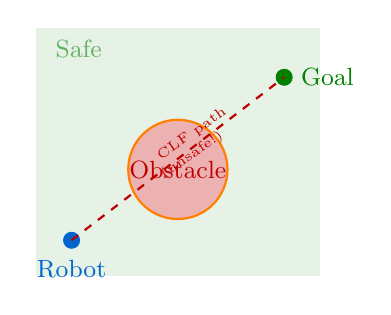
\begin{tikzpicture}[scale=0.9]
    % Safe region
    \fill[accentgreen!10] (0,0) rectangle (4,3.5);
    \node[accentgreen!60, font=\small] at (0.6,3.2) {Safe};
    
    % Obstacle
    \fill[accentred!30] (2,1.5) circle (0.7);
    \draw[thick, accentorange] (2,1.5) circle (0.7);
    \node[accentred, font=\small] at (2,1.5) {Obstacle};
    
    % Goal
    \fill[accentgreen] (3.5,2.8) circle (0.12);
    \node[accentgreen, right, font=\small] at (3.6,2.8) {Goal};
    
    % Robot
    \fill[brightblue] (0.5,0.5) circle (0.12);
    \node[brightblue, below, font=\small] at (0.5,0.35) {Robot};
    
    % Unsafe path
    \draw[thick, accentred, dashed] (0.5,0.5) -- (3.5,2.8);
    \node[accentred, font=\tiny, rotate=35] at (2.2,2) {CLF path};
    \node[accentred, font=\tiny, rotate=35] at (2.2,1.7) {(unsafe!)};
\end{tikzpicture}
\end{columns}

\vspace{0.3cm}

\begin{alertblock}{Critical Gap}
CLF controller chooses shortest path to goal, even through obstacles. Need additional framework for safety.
\end{alertblock}

\end{frame}

% ================================================================
\begin{frame}{Control Barrier Functions}

\textbf{Approach:} Define barrier function $h(\xv)$ encoding safe set

\vspace{0.4cm}

\textbf{Interpretation:}
\begin{align*}
h(\xv) > 0 &\Rightarrow \text{SAFE} \\
h(\xv) = 0 &\Rightarrow \text{BOUNDARY} \\
h(\xv) < 0 &\Rightarrow \text{UNSAFE}
\end{align*}

\vspace{0.3cm}

\textbf{Safe Set:}
\[
\mathcal{C} = \{\xv \in \mathbb{R}^n : h(\xv) \geq 0\}
\]

\vspace{0.3cm}

\textbf{Objective:} Keep $\xv(t) \in \mathcal{C}$ for all $t$ \quad (forward invariance)

\end{frame}

% ================================================================
\begin{frame}{CBF: Visual Interpretation}

\centering
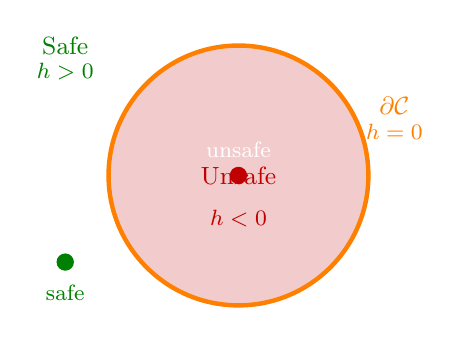
\begin{tikzpicture}[scale=1.1]
    % Unsafe region (interior of circle = obstacle)
    \fill[accentred!20] (2.5,2) circle (1.5);
    \node[accentred, font=\small] at (2.5,2) {Unsafe};
    \node[accentred, font=\footnotesize] at (2.5,1.5) {$h < 0$};
    
    % Boundary
    \draw[ultra thick, accentorange] (2.5,2) circle (1.5);
    \node[accentorange, font=\small] at (4.3,2.8) {$\partial\mathcal{C}$};
    \node[accentorange, font=\footnotesize] at (4.3,2.5) {$h = 0$};
    
    % Safe region label
    \node[accentgreen, font=\small] at (0.5,3.5) {Safe};
    \node[accentgreen, font=\footnotesize] at (0.5,3.2) {$h > 0$};
    
    % Safe point
    \fill[accentgreen] (0.5,1) circle (0.1);
    \node[accentgreen, below, font=\footnotesize] at (0.5,0.85) {safe};
    
    % Unsafe point
    \fill[accentred] (2.5,2) circle (0.1);
    \node[white, font=\footnotesize] at (2.5,2.3) {unsafe};
\end{tikzpicture}

\end{frame}

% ================================================================
\begin{frame}{CBF Requirements}

\begin{block}{Control Barrier Function}
\begin{enumerate}
    \item \textbf{Safe Set:} $\mathcal{C} = \{\xv \in D : h(\xv) \geq 0\}$
    
    \vspace{0.3cm}
    
    \item \textbf{Boundary:} $\partial\mathcal{C} = \{\xv : h(\xv) = 0\}$
    
    \vspace{0.3cm}
    
    \item \textbf{Interior:} $\text{Int}(\mathcal{C}) = \{\xv : h(\xv) > 0\}$
\end{enumerate}
\end{block}

\vspace{0.4cm}

Function must equal zero \textbf{only} on boundary

\vspace{0.5cm}

\begin{block}{Forward Invariance}
Set $\mathcal{C}$ is \textbf{forward invariant} if:

\vspace{0.2cm}

For all $\xv(t_0) \in \mathcal{C}$ and all $t \geq t_0$: $\xv(t) \in \mathcal{C}$
\end{block}

\end{frame}

% ================================================================
\begin{frame}{CBF Safety Condition}

To guarantee forward invariance:

\begin{equation}
\dot{h}(\xv, \uv) \geq -\alpha(h(\xv))
\end{equation}

where $\alpha : \mathbb{R} \rightarrow \mathbb{R}$ is extended class-$\mathcal{K}$ (commonly $\alpha(h) = \gamma h$, $\gamma > 0$)

\vspace{0.5cm}

\begin{block}{CBF Safety Condition}
\[
\dot{h}(\xv, \uv) \geq -\alpha(h(\xv))
\]
\end{block}

\vspace{0.4cm}

\textbf{At boundary:} $\dot{h} \geq 0$ (cannot decrease into unsafe region)

\vspace{0.4cm}

This inequality, when satisfied, \textbf{mathematically guarantees safety}

\end{frame}

% ================================================================
\begin{frame}{Understanding the CBF Condition}

\textbf{Condition:} $\dot{h}(\xv, \uv) \geq -\alpha(h(\xv))$

\vspace{0.5cm}

\begin{block}{Case 1: At Boundary ($h = 0$)}
\[
\dot{h} \geq -\alpha(0) = 0
\]

Time derivative must be non-negative. Robot can:
\begin{itemize}
    \item Move tangent to boundary ($\dot{h} = 0$)
    \item Move away from danger ($\dot{h} > 0$)
\end{itemize}

Movement into unsafe region ($\dot{h} < 0$) is \textbf{prohibited}
\end{block}

\vspace{0.3cm}

\begin{block}{Case 2: In Interior ($h > 0$)}
\[
\dot{h} \geq -\alpha(h) < 0
\]

Some decrease allowed (can approach boundary), but rate limited
\end{block}

\end{frame}

% ================================================================
\begin{frame}{CBF Design Examples}

\begin{columns}[T]
\column{0.48\textwidth}
\textbf{Example 1: Adaptive Cruise}

Maintain safe following distance:
\[
h_1 = D - \tau V_{\text{rel}}
\]

\begin{itemize}
    \item $D$: inter-vehicle distance
    \item $\tau$: time headway
    \item $V_{\text{rel}}$: relative velocity
\end{itemize}

\vspace{0.5cm}

\textbf{Example 2: Lane Keeping}
\[
h_2 = d - \frac{\sin(\theta) y_{\text{ref}}}{V^2}
\]

\column{0.48\textwidth}
\textbf{Example 3: Pendulum Angle}

\centering
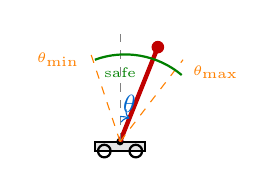
\begin{tikzpicture}[scale=0.8]
    % Cart
    \draw[thick, fill=gray!20] (-0.4,-0.15) rectangle (0.4,0);
    \draw[thick] (-0.25,-0.15) circle (0.1);
    \draw[thick] (0.25,-0.15) circle (0.1);
    
    % Pivot
    \fill[black] (0,0) circle (0.06);
    
    % Pendulum
    \draw[ultra thick, accentred] (0,0) -- (0.6,1.5);
    \fill[accentred] (0.6,1.5) circle (0.1);
    
    % Angle
    \draw[->, brightblue] (0,0.4) arc (90:68:0.4);
    \node[brightblue, font=\small] at (0.15,0.6) {$\theta$};
    
    % Vertical reference
    \draw[dashed, gray] (0,0) -- (0,1.8);
    
    % Constraints
    \draw[dashed, accentorange] (0,0) -- (-0.5,1.5);
    \node[accentorange, font=\tiny, left] at (-0.5,1.3) {$\theta_{\min}$};
    \draw[dashed, accentorange] (0,0) -- (1,1.3);
    \node[accentorange, font=\tiny, right] at (1,1.1) {$\theta_{\max}$};
    
    % Safe arc
    \draw[thick, accentgreen] (-0.4,1.3) arc (110:50:1.4);
    \node[accentgreen, font=\tiny] at (0,1.1) {safe};
\end{tikzpicture}

\vspace{0.3cm}

\begin{align*}
h_1 &= \theta - \theta_{\min} \geq 0 \\
h_2 &= -\theta + \theta_{\max} \geq 0
\end{align*}
\end{columns}

\end{frame}

% ================================================================
\begin{frame}{Homework: Circular Obstacle}

\textbf{Problem:} Avoid circular obstacle

\vspace{0.3cm}

\begin{columns}[T]
\column{0.48\textwidth}
\textbf{Setup:}
\begin{itemize}
    \item Obstacle center: $(x_{\text{obs}}, y_{\text{obs}})$
    \vspace{0.2cm}
    \item Obstacle radius: $r_{\text{obs}}$
    \vspace{0.2cm}
    \item Robot radius: $r_{\text{robot}}$
    \vspace{0.2cm}
    \item Safety radius:
\end{itemize}
\[
r_{\text{safe}} = r_{\text{obs}} + r_{\text{robot}}
\]

\vspace{0.3cm}

\textbf{Barrier Function:}
\[
h = (x - x_{\text{obs}})^2 + (y - y_{\text{obs}})^2 - r_{\text{safe}}^2
\]

\column{0.48\textwidth}
\centering
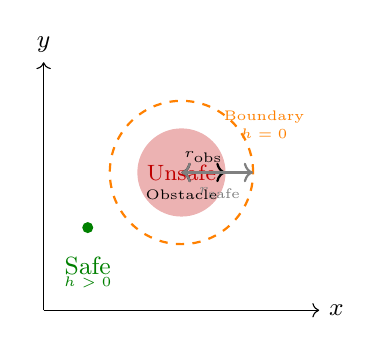
\begin{tikzpicture}[scale=0.7]
    % Axes
    \draw[->] (0,0) -- (5,0) node[right, font=\small] {$x$};
    \draw[->] (0,0) -- (0,4.5) node[above, font=\small] {$y$};
    
    % Obstacle
    \fill[accentred!30] (2.5,2.5) circle (0.8);
    \node[accentred, font=\footnotesize] at (2.5,2.5) {Unsafe};
    \node[font=\tiny] at (2.5,2.1) {Obstacle};
    
    % Safe boundary
    \draw[dashed, accentorange, thick] (2.5,2.5) circle (1.3);
    \node[accentorange, font=\tiny] at (4,3.5) {Boundary};
    \node[accentorange, font=\tiny] at (4,3.2) {$h = 0$};
    
    % Safe region label
    \node[accentgreen, font=\small] at (0.8,0.8) {Safe};
    \node[accentgreen, font=\tiny] at (0.8,0.5) {$h > 0$};
    
    % Safe point
    \fill[accentgreen] (0.8,1.5) circle (0.1);
    
    % Radius annotations
    \draw[<->, thick] (2.5,2.5) -- (3.3,2.5);
    \node[font=\tiny, above] at (2.9,2.5) {$r_{\text{obs}}$};
    \draw[<->, thick, gray] (2.5,2.5) -- (3.8,2.5);
    \node[font=\tiny, below, gray] at (3.2,2.4) {$r_{\text{safe}}$};
\end{tikzpicture}

\vspace{0.2cm}

\textbf{Safe Region}
\end{columns}

\end{frame}

% ================================================================
% PART 6: LIE DERIVATIVES
% ================================================================
\section{Lie Derivatives}

\begin{frame}{The Tractability Challenge}

Two constraints established:

\vspace{0.3cm}

\begin{align}
\text{Stability (CLF):} \quad & \dot{V}(\xv, \uv) \leq -\gamma V(\xv) \\[0.3cm]
\text{Safety (CBF):} \quad & \dot{h}(\xv, \uv) \geq -\alpha(h(\xv))
\end{align}

\vspace{0.4cm}

\textbf{Challenge:} Both $\dot{V}$ and $\dot{h}$ are complex nonlinear functions of $\xv$ and $\uv$

\vspace{0.5cm}

\begin{alertblock}{Key Question}
How to compute and solve efficiently in real-time (100+ Hz)?
\end{alertblock}

\vspace{0.4cm}

\textbf{Solution:} Exploit \textbf{control-affine structure} using \textbf{Lie derivatives}

\end{frame}

% ================================================================
\begin{frame}{Control-Affine Systems}

Most robotic systems have \textbf{control-affine form}:

\begin{equation}
\dot{\xv} = f(\xv) + g(\xv)\uv
\end{equation}

\vspace{0.4cm}

\textbf{Components:}
\begin{itemize}
    \item $f(\xv)$: Drift vector field (evolution with $\uv = 0$)
    \vspace{0.2cm}
    \item $g(\xv)$: Control influence matrix (maps control to state velocity)
\end{itemize}

\vspace{0.5cm}

\textbf{Differential Drive Example:}
\[
\begin{bmatrix} \dot{x} \\ \dot{y} \\ \dot{\theta} \end{bmatrix} = 
\underbrace{\begin{bmatrix} 0 \\ 0 \\ 0 \end{bmatrix}}_{f(\xv)} + 
\underbrace{\begin{bmatrix} \cos\theta & 0 \\ \sin\theta & 0 \\ 0 & 1 \end{bmatrix}}_{g(\xv)}
\begin{bmatrix} v \\ \omega \end{bmatrix}
\]

\vspace{0.2cm}

This is \textbf{driftless} ($f = 0$)

\end{frame}

% ================================================================
\begin{frame}{Deriving Time Derivatives}

\textbf{Chain Rule for $\dot{h}$:}

\vspace{0.3cm}

\[
\dot{h} = \frac{dh}{dt} = \frac{\partial h}{\partial \xv} \dot{\xv}
\]

\vspace{0.3cm}

\[
\dot{h} = \frac{\partial h}{\partial \xv} [f(\xv) + g(\xv)\uv]
\]

\vspace{0.3cm}

\[
\dot{h} = \underbrace{\frac{\partial h}{\partial \xv} f(\xv)}_{\text{drift term}} + \underbrace{\frac{\partial h}{\partial \xv} g(\xv)}_{\text{control term}} \uv
\]

\vspace{0.5cm}

\begin{block}{Key Result}
Control $\uv$ now appears \textbf{linearly}!
\end{block}

\end{frame}

% ================================================================
\begin{frame}{Lie Derivative Notation}

Standard names from geometric control:

\vspace{0.4cm}

\begin{block}{Lie Derivative Definitions}
\textbf{Lie derivative of $h$ along $f$:}
\[
L_f h(\xv) := \frac{\partial h}{\partial \xv} f(\xv)
\]

Rate of change due to natural drift

\vspace{0.4cm}

\textbf{Lie derivative of $h$ along $g$:}
\[
L_g h(\xv) := \frac{\partial h}{\partial \xv} g(\xv)
\]

How control $\uv$ influences rate of change of $h$
\end{block}

\end{frame}

% ================================================================
\begin{frame}{The Power of Lie Derivatives}

At any fixed state $\xv$, Lie derivatives are \textbf{constants}:

\vspace{0.3cm}

\begin{itemize}
    \item $L_f h(\xv)$ is a \textbf{scalar}
    \vspace{0.2cm}
    \item $L_g h(\xv)$ is a \textbf{row vector}
    \vspace{0.2cm}
    \item $h(\xv)$ is a \textbf{scalar}
\end{itemize}

\vspace{0.5cm}

\begin{block}{Linear Constraints}
\textbf{Original (nonlinear):}
\[
\dot{h}(\xv, \uv) \geq -\alpha(h(\xv))
\]

\textbf{With Lie derivatives (linear in $\uv$):}
\[
L_f h(\xv) + L_g h(\xv) \uv \geq -\alpha(h(\xv))
\]

\textbf{Rearranged:}
\[
L_g h(\xv) \uv \geq -\alpha(h(\xv)) - L_f h(\xv)
\]
\end{block}

\end{frame}

% ================================================================
\begin{frame}{Computation Example}

\textbf{System:} Differential drive, $\xv = [x, y, \theta]^T$, $\uv = [v, \omega]^T$

\vspace{0.3cm}

\textbf{Dynamics:} $f(\xv) = 0$, \quad $g(\xv) = \begin{bmatrix} \cos\theta & 0 \\ \sin\theta & 0 \\ 0 & 1 \end{bmatrix}$

\vspace{0.3cm}

\textbf{Barrier:} Circular obstacle
\[
h = (x - x_{\text{obs}})^2 + (y - y_{\text{obs}})^2 - r_{\text{safe}}^2
\]

\vspace{0.3cm}

\textbf{Gradient:}
\[
\nabla h = \begin{bmatrix} 2(x - x_{\text{obs}}) & 2(y - y_{\text{obs}}) & 0 \end{bmatrix}
\]

\vspace{0.3cm}

\textbf{Lie Derivatives:}
\begin{align*}
L_f h &= \nabla h \cdot f = 0 \\
L_g h &= \begin{bmatrix} 2(x - x_{\text{obs}})\cos\theta + 2(y - y_{\text{obs}})\sin\theta & 0 \end{bmatrix}
\end{align*}

\textbf{Note:} Only $v$ appears; $\omega$ has no direct effect on distance

\end{frame}

% ================================================================
% PART 7: CLF-CBF QP
% ================================================================
\section{CLF-CBF Quadratic Programming}

\begin{frame}{The Control Hierarchy}

\textbf{At time $t$, we have:}
\begin{itemize}
    \item Current state $\xv(t)$
    \vspace{0.2cm}
    \item Desired control $\uv_{\text{des}}$ from NMPC
    \vspace{0.2cm}
    \item CLF constraint: $L_f V + L_g V \cdot \uv \leq -\gamma V$
    \vspace{0.2cm}
    \item CBF constraint: $L_f h + L_g h \cdot \uv \geq -\alpha h$
\end{itemize}

\vspace{0.4cm}

\begin{alertblock}{Potential Conflicts}
\begin{enumerate}
    \item What if $\uv_{\text{des}}$ violates safety?
    \item What if safety and stability incompatible?
    \item How to prioritize?
\end{enumerate}
\end{alertblock}

\vspace{0.3cm}

\textbf{Solution:} Real-time optimization with Safety (hard), Stability (soft), Stay close to $\uv_{\text{des}}$ (objective)

\end{frame}

% ================================================================
\begin{frame}{Why Quadratic Programming?}

\begin{columns}[T]
\column{0.5\textwidth}
\textbf{Problem Structure:}

\vspace{0.3cm}

\begin{itemize}
    \item \textbf{Objective:} Quadratic $\|\uv - \uv_{\text{des}}\|^2$
    \vspace{0.2cm}
    \item \textbf{Constraints:} Linear (via Lie derivatives)
    \vspace{0.2cm}
    \item \textbf{Result:} Convex QP
\end{itemize}

\vspace{0.4cm}

\textbf{Properties:}
\begin{itemize}
    \item Global optimum
    \vspace{0.2cm}
    \item Polynomial-time
    \vspace{0.2cm}
    \item Microsecond-scale
    \vspace{0.2cm}
    \item Well-studied algorithms
\end{itemize}

\column{0.45\textwidth}
\centering
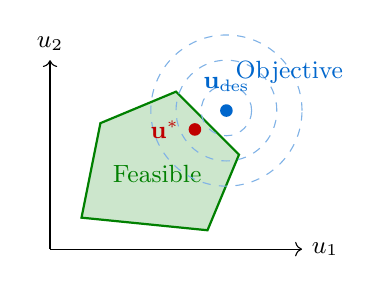
\begin{tikzpicture}[scale=0.8]
    % Feasible region
    \fill[accentgreen!20] (0.5,0.5) -- (2.5,0.3) -- (3,1.5) -- (2,2.5) -- (0.8,2) -- cycle;
    \draw[thick, accentgreen] (0.5,0.5) -- (2.5,0.3) -- (3,1.5) -- (2,2.5) -- (0.8,2) -- cycle;
    \node[accentgreen, font=\small] at (1.7,1.2) {Feasible};
    
    % Objective contours
    \draw[dashed, brightblue!50] (2.8,2.2) circle (0.4);
    \draw[dashed, brightblue!50] (2.8,2.2) circle (0.8);
    \draw[dashed, brightblue!50] (2.8,2.2) circle (1.2);
    \node[brightblue, font=\small] at (3.8,2.8) {Objective};
    
    % Desired point (outside)
    \fill[brightblue] (2.8,2.2) circle (0.1);
    \node[brightblue, above, font=\small] at (2.8,2.35) {$\uv_{\text{des}}$};
    
    % Optimal point
    \fill[accentred] (2.3,1.9) circle (0.1);
    \node[accentred, left, font=\small] at (2.2,1.9) {$\uv^*$};
    
    % Axes
    \draw[->] (0,0) -- (4,0) node[right, font=\small] {$u_1$};
    \draw[->] (0,0) -- (0,3) node[above, font=\small] {$u_2$};
\end{tikzpicture}
\end{columns}

\end{frame}

% ================================================================
\begin{frame}{Naive Formulation}

\textbf{Initial attempt:}

\vspace{0.3cm}

\[
\min_{\uv} \quad \frac{1}{2}\|\uv - \uv_{\text{des}}\|^2
\]

\vspace{0.2cm}

subject to:
\begin{align}
L_g h(\xv) \uv &\geq -\alpha(h) - L_f h && \text{(Safety: CBF)} \\
L_g V(\xv) \uv &\leq -\gamma V - L_f V && \text{(Stability: CLF)} \\
\uv_{\min} \leq \uv &\leq \uv_{\max} && \text{(Actuator limits)}
\end{align}

\vspace{0.4cm}

\begin{alertblock}{Feasibility Problem}
This can be \textbf{infeasible}. If goal is behind obstacle, no control can simultaneously maintain safety and ensure stability. QP fails!
\end{alertblock}

\end{frame}

% ================================================================
\begin{frame}{Slack Variable Technique}

\textbf{Solution:} Make CLF constraint ``soft'' with relaxation variable

\vspace{0.4cm}

\begin{block}{Control Hierarchy}
\begin{enumerate}
    \item \textbf{Safety (highest):} Hard constraint --- always holds
    \vspace{0.2cm}
    \item \textbf{Stability (secondary):} Soft constraint --- relaxed when necessary
    \vspace{0.2cm}
    \item \textbf{Performance:} Objective --- minimize deviation from $\uv_{\text{des}}$
\end{enumerate}
\end{block}

\vspace{0.4cm}

\textbf{Implementation:} Introduce slack $\delta \geq 0$

\vspace{0.3cm}

\textbf{Modified CLF:}
\[
L_g V \cdot \uv \leq -\gamma V - L_f V + \delta
\]

\begin{itemize}
    \item $\delta = 0$: Original CLF satisfied
    \item $\delta > 0$: Stability relaxed (safety priority)
\end{itemize}

\end{frame}

% ================================================================
\begin{frame}{Final CLF-CBF-QP}

\begin{block}{Complete Optimization}
Find optimal $(\uv^*, \delta^*)$:

\vspace{0.3cm}

\[
\min_{\uv, \delta} \quad \frac{1}{2}\|\uv - \uv_{\text{des}}\|^2 + \frac{p}{2}\delta^2
\]

\vspace{0.2cm}

subject to:
\begin{align*}
L_g h \cdot \uv &\geq -\alpha(h) - L_f h && \textbf{(HARD: Safety)} \\
L_g V \cdot \uv &\leq -\gamma V - L_f V + \delta && \text{(Soft: Stability)} \\
\uv_{\min} \leq \uv &\leq \uv_{\max}, \quad \delta \geq 0
\end{align*}

where $p \gg 1$ (typically $10^3$ to $10^4$)
\end{block}

\vspace{0.3cm}

Large $p$ ensures $\delta$ minimized. Stability violated \textit{only} when necessary for safety.

\end{frame}

% ================================================================
% PART 8: TWO-LAYER ARCHITECTURE
% ================================================================
\section{Two-Layer Architecture}

\begin{frame}{Layered Strategy}

\textbf{Philosophy:} Separate \textit{performance} from \textit{safety}

\vspace{0.4cm}

\begin{columns}[T]
\column{0.48\textwidth}
\begin{block}{Layer 1: NMPC}
\begin{itemize}
    \item Rate: 10--50 Hz
    \vspace{0.2cm}
    \item Complex, non-convex
    \vspace{0.2cm}
    \item Horizon: 1--2 sec
    \vspace{0.2cm}
    \item Output: $\uv_{\text{des}}$
    \vspace{0.2cm}
    \item \textcolor{accentred}{Untrusted}
\end{itemize}
\end{block}

\column{0.48\textwidth}
\begin{block}{Layer 2: ASIF}
\begin{itemize}
    \item Rate: 100--1000 Hz
    \vspace{0.2cm}
    \item Fast QP (convex)
    \vspace{0.2cm}
    \item Instantaneous
    \vspace{0.2cm}
    \item Output: $\uv_{\text{act}}$
    \vspace{0.2cm}
    \item \textcolor{accentgreen}{Trusted}
\end{itemize}
\end{block}
\end{columns}

\vspace{0.4cm}

\textbf{Advantage:} Use sophisticated (unreliable) planning while maintaining provable safety

\end{frame}

% ================================================================
\begin{frame}{ASIF Safety Filter}

\centering
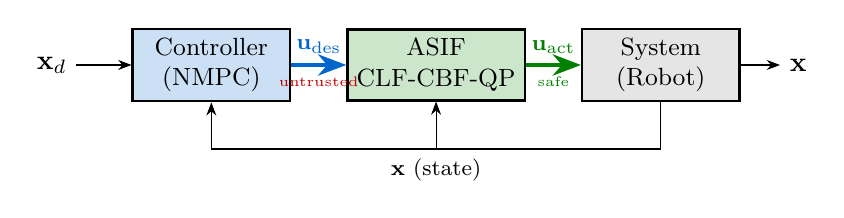
\begin{tikzpicture}[scale=0.85, >=Stealth,
    block/.style={draw, rectangle, minimum width=2cm, minimum height=0.9cm, align=center, font=\small, thick}]
    
    \node (xd) {$\xv_d$};
    \node[block, fill=brightblue!20, right=0.7cm of xd] (ctrl) {Controller\\(NMPC)};
    \node[block, fill=accentgreen!20, right=0.7cm of ctrl] (asif) {ASIF\\CLF-CBF-QP};
    \node[block, fill=gray!20, right=0.7cm of asif] (sys) {System\\(Robot)};
    \node[right=0.5cm of sys] (x) {$\xv$};
    
    \draw[->] (xd) -- (ctrl);
    \draw[->, ultra thick, brightblue] (ctrl) -- node[above, font=\footnotesize] {$\uv_{\text{des}}$} node[below, font=\tiny, accentred] {untrusted} (asif);
    \draw[->, ultra thick, accentgreen] (asif) -- node[above, font=\footnotesize] {$\uv_{\text{act}}$} node[below, font=\tiny, accentgreen] {safe} (sys);
    \draw[->] (sys) -- (x);
    
    \draw[->] (sys.south) -- ++(0,-0.7) -| node[pos=0.25, below, font=\footnotesize] {$\xv$ (state)} (ctrl.south);
    \draw[->] (sys.south) -- ++(0,-0.7) -| (asif.south);
\end{tikzpicture}

\vspace{0.5cm}

\begin{block}{ASIF Cycle}
\begin{enumerate}
    \item Receive $\uv_{\text{des}}$ and $\xv$
    \item Compute Lie derivatives
    \item Formulate CLF-CBF-QP
    \item Solve QP ($< 1$ ms)
    \item Output safe $\uv_{\text{act}}$
\end{enumerate}
\end{block}

\end{frame}

% ================================================================
\begin{frame}{Complete System Architecture}

\centering
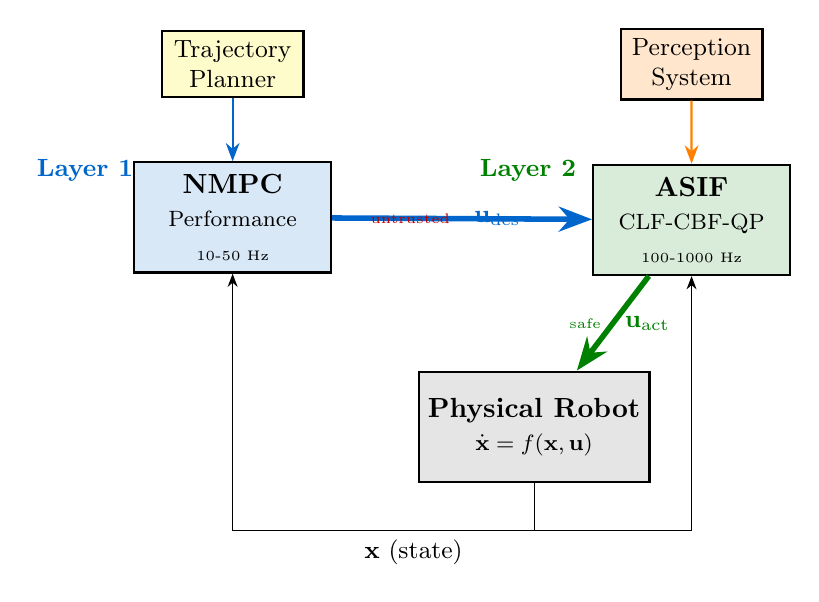
\begin{tikzpicture}[scale=0.75, >=Stealth,
    block/.style={draw, rectangle, minimum width=1.8cm, minimum height=0.8cm, align=center, font=\small, thick},
    bigblock/.style={draw, rectangle, minimum width=2.5cm, minimum height=1.4cm, align=center, thick, font=\normalsize}]
    
    % Top inputs
    \node[block, fill=yellow!20] (planner) {Trajectory\\Planner};
    \node[block, fill=accentorange!20, right=4cm of planner] (perception) {Perception\\System};
    
    % NMPC layer
    \node[bigblock, fill=brightblue!15, below=0.8cm of planner] (nmpc) {\textbf{NMPC}\\{\footnotesize Performance}\\{\tiny 10-50 Hz}};
    
    % ASIF layer
    \node[bigblock, fill=accentgreen!15, below=0.8cm of perception] (asif) {\textbf{ASIF}\\{\footnotesize CLF-CBF-QP}\\{\tiny 100-1000 Hz}};
    
    % Robot
    \node[bigblock, fill=gray!20, below=1.2cm of asif, xshift=-2cm] (robot) {\textbf{Physical Robot}\\{\footnotesize $\dot{\xv} = f(\xv, \uv)$}};
    
    % Connections
    \draw[->, thick, brightblue] (planner) -- (nmpc);
    \draw[->, thick, accentorange] (perception) -- (asif);
    \draw[->, ultra thick, brightblue, line width=2pt] (nmpc) -- node[right, font=\small] {$\uv_{\text{des}}$} node[left, font=\tiny, accentred] {untrusted} (asif);
    \draw[->, ultra thick, accentgreen, line width=2pt] (asif) -- node[right, font=\small] {$\uv_{\text{act}}$} node[left, font=\tiny, accentgreen] {safe} (robot);
    
    % Feedback
    \draw[->] (robot.south) -- ++(0,-0.8) -| node[pos=0.2, below, font=\small] {$\xv$ (state)} (nmpc.south);
    \draw[->] (robot.south) -- ++(0,-0.8) -| (asif.south);
    
    % Layer labels
    \node[font=\small, brightblue] at (-2.5,-1.8) {\textbf{Layer 1}};
    \node[font=\small, accentgreen] at (5,-1.8) {\textbf{Layer 2}};
\end{tikzpicture}

\vspace{0.3cm}

State feedback $\xv$ to both layers. \textbf{ASIF has final authority.}

\end{frame}

% ================================================================
\begin{frame}{ASIF: Benefits and Limitations}

\begin{columns}[T]
\column{0.48\textwidth}
\textbf{Advantages:}
\begin{itemize}
    \item Microsecond computation
    \vspace{0.2cm}
    \item Formal safety guarantee
    \vspace{0.2cm}
    \item Modular architecture
    \vspace{0.2cm}
    \item Minimal intervention
    \vspace{0.2cm}
    \item Works with any planner
\end{itemize}

\vspace{0.3cm}

Can use learning-based policies, game theory, or human teleoperation with safety enforced

\column{0.48\textwidth}
\textbf{Limitations:}
\begin{itemize}
    \item Performance layer safety-ignorant
    \vspace{0.2cm}
    \item May generate unsafe commands
    \vspace{0.2cm}
    \item Frequent intervention reduces efficiency
    \vspace{0.2cm}
    \item No conflict resolution
\end{itemize}

\vspace{0.4cm}

\textbf{Alternative:}

Safety-Aware NMPC embeds CBF directly in optimization
\end{columns}

\end{frame}

% ================================================================
% PART 9: MODEL UNCERTAINTY
% ================================================================
\section{Model Uncertainty}

\begin{frame}{The Critical Assumption}

\begin{alertblock}{Assumption So Far}
\textbf{Perfect system model:}
\[
\dot{\xv} = f(\xv, \uv)
\]
\end{alertblock}

\vspace{0.4cm}

\textbf{Reality:} All models are wrong

\[
\dot{\xv}_{\text{true}} = f(\xv, \uv) + d(\xv, t)
\]

\vspace{0.4cm}

\textbf{Sources of $d$:}

\begin{columns}[T]
\column{0.48\textwidth}
\begin{itemize}
    \item Wheel slip
    \item Unknown mass
    \item Wind disturbances
\end{itemize}

\column{0.48\textwidth}
\begin{itemize}
    \item Actuator delays
    \item Sensor noise
    \item Friction models
\end{itemize}
\end{columns}

\end{frame}

% ================================================================
\begin{frame}{Why Model Error Breaks Safety}

\textbf{CBF condition:}
\[
\dot{h} = L_f h + L_g h \cdot \uv \geq -\alpha(h)
\]

\vspace{0.3cm}

\textbf{With model error:}
\[
\dot{h}_{\text{true}} = L_f h + L_g h \cdot \uv + \underbrace{\frac{\partial h}{\partial \xv} d}_{\text{unknown disturbance}}
\]

\vspace{0.4cm}

\begin{alertblock}{Safety Guarantee Voided}
\begin{itemize}
    \item We compute $L_f h$, $L_g h$ using incorrect model $f$
    \vspace{0.2cm}
    \item True system evolves according to $f + d$
    \vspace{0.2cm}
    \item QP solution may not satisfy true safety condition
    \vspace{0.2cm}
    \item \textbf{Mathematical guarantee no longer holds}
\end{itemize}
\end{alertblock}

\end{frame}

% ================================================================
\begin{frame}{Robust Safety Approaches}

\textbf{Three Research Directions:}

\vspace{0.3cm}

\begin{block}{1. Robust CBF (Worst-Case)}
If $\|d\| \leq d_{\max}$, modify safety:
\[
L_g h \cdot \uv \geq -\alpha(h) - L_f h + \|\nabla h\| d_{\max}
\]

\textbf{Trade-off:} Conservative (reduces performance)
\end{block}

\vspace{0.3cm}

\begin{block}{2. Adaptive CBF (Learning)}
Estimate $d(\xv, t)$ in real-time using:
\begin{itemize}
    \item Extended Kalman Filters
    \item Gaussian Process Regression
    \item Neural network observers
\end{itemize}
\end{block}

\end{frame}

% ================================================================
\begin{frame}{Learning-Based Safe Control}

\begin{block}{3. Reinforcement Learning + CBF}
\textbf{Concept:} Combine learning flexibility with formal safety

\vspace{0.3cm}

\begin{itemize}
    \item \textbf{RL Agent:} Learns optimal policies from experience
    \vspace{0.2cm}
    \item \textbf{CBF-QP Filter:} Ensures safety during exploration
    \vspace{0.2cm}
    \item \textbf{Result:} Safe learning without crashes
\end{itemize}
\end{block}

\vspace{0.4cm}

\centering
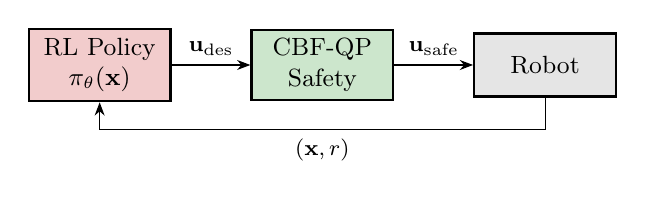
\begin{tikzpicture}[scale=0.8, >=Stealth,
    block/.style={draw, rectangle, minimum width=1.8cm, minimum height=0.8cm, align=center, font=\small, thick}]
    
    \node[block, fill=accentred!20] (rl) {RL Policy\\$\pi_\theta(\xv)$};
    \node[block, fill=accentgreen!20, right=1cm of rl] (cbf) {CBF-QP\\Safety};
    \node[block, fill=gray!20, right=1cm of cbf] (robot) {Robot};
    
    \draw[->] (rl) -- node[above, font=\footnotesize] {$\uv_{\text{des}}$} (cbf);
    \draw[->] (cbf) -- node[above, font=\footnotesize] {$\uv_{\text{safe}}$} (robot);
    \draw[->] (robot.south) -- ++(0,-0.5) -| node[pos=0.25, below, font=\footnotesize] {$(\xv, r)$} (rl.south);
\end{tikzpicture}

\end{frame}

% ================================================================
% PART 10: HOMEWORK
% ================================================================
\section{Homework}

\begin{frame}{Homework Assignment}

\begin{block}{Overview}
Apply Control Barrier Functions to ensure safe robot navigation around a pedestrian.
\end{block}

\vspace{0.4cm}

\textbf{Requirements:}

\vspace{0.3cm}

\begin{enumerate}
    \item \textbf{Scenario:} Robot must reach goal while avoiding pedestrian obstacle
    
    \vspace{0.3cm}
    
    \item \textbf{Define geometric constraint:}
    \[
    h() = \|\text{robot} - \text{pedestrian}\| - d_{\text{safe}} \geq 0
    \]
    
    \vspace{0.3cm}
    
    \item \textbf{Apply CBF approach:} Use Control Barrier Function to guarantee safety
    
    \vspace{0.3cm}
    
    \item \textbf{Write 5 equations:} System dynamics, barrier function, CBF condition, control bounds, distance formula
    
    \vspace{0.3cm}
    
    \item \textbf{Show solution:} Demonstrate robot reaches goal while maintaining safe distance from pedestrian
\end{enumerate}

\end{frame}

% ================================================================
% SUMMARY
% ================================================================
\section{Summary}

\begin{frame}{Lecture Summary}

\textbf{Key Concepts Covered:}

\vspace{0.4cm}

\begin{enumerate}
    \item \textbf{Fundamental Challenge:} Performance vs.\ Safety tradeoff
    
    \vspace{0.3cm}
    
    \item \textbf{NMPC:} Prediction-based optimization for performance
    
    \vspace{0.3cm}
    
    \item \textbf{CLF:} Control Lyapunov Functions for stability guarantees
    
    \vspace{0.3cm}
    
    \item \textbf{CBF:} Control Barrier Functions for safety guarantees
    
    \vspace{0.3cm}
    
    \item \textbf{Lie Derivatives:} Transform nonlinear constraints to linear
    
    \vspace{0.3cm}
    
    \item \textbf{CLF-CBF-QP:} Real-time safe control via quadratic programming
    
    \vspace{0.3cm}
    
    \item \textbf{Two-Layer Architecture:} NMPC + ASIF for safe autonomy
\end{enumerate}

\end{frame}

% ================================================================
\begin{frame}{Key Takeaways}

\begin{block}{Framework Hierarchy}
\begin{enumerate}
    \item \textbf{Safety:} CBF constraint (HARD) --- never violated
    \vspace{0.2cm}
    \item \textbf{Stability:} CLF constraint (soft) --- relaxed when needed
    \vspace{0.2cm}
    \item \textbf{Performance:} Minimize $\|\uv - \uv_{\text{des}}\|^2$
\end{enumerate}
\end{block}

\vspace{0.4cm}

\begin{block}{Design Principles}
\begin{itemize}
    \item Lie derivatives make constraints linear in control
    \vspace{0.2cm}
    \item Slack variables ensure QP feasibility
    \vspace{0.2cm}
    \item Two-layer architecture separates concerns
    \vspace{0.2cm}
    \item Model accuracy is critical for guarantees
\end{itemize}
\end{block}

\end{frame}

% ================================================================
% END SLIDE
% ================================================================
{
\setbeamertemplate{footline}{}
\begin{frame}[plain]
\begin{center}
\vspace{2cm}

{\Large\bfseries End of Lecture 7}

\vspace{1.5cm}

{\large Questions?}

\vspace{2cm}

\textcolor{nyupurple}{\textbf{Next:} Motion Planning Algorithms}

\end{center}
\end{frame}
}

\end{document}
